%Yes, you've got it right: it's my work-to-rule strike against idiocy.
\chapter{Охрана труда}
Осознавая первоочередную важность сохранения жизни и здоровья пользователей любой системы и первоочередной приоритет требований безопасности перед всеми остальными, рассмотрим, прежде, чем начинать разработку, какой потенциальный вред пользователю может нанести подобная система.

Все виды опасностей на производстве можно разделить на следующие виды\cite{enwikiosh}:
\begin{enumerate}
	\item
		Механические, такие как удары, падения, поражения высоким давлением, а также иные физические, такие как свет, ионизирующее излучение, звук, электрический ток и тому подобные;
	\item
		Биологические, такие как вирусы, бактерии, грибки, паразиты и так далее;
	\item
		Химические, такие как кислоты, основания, тяжёлые металлы и другие;
	\item
		Заболевания опорно-двигательного аппарата;
	\item
		Психологические, такие как моббинг\cite{enwikimobbing}, эмоциональное выгорание\cite{enwikiburnout}, негативное воздействие среды, принуждающей к нездоровой активности (такой как неумеренное употребление спиртных напитков, курение и так далее) как необходимому условию карьерного роста и интеграции в коллектив.
\end{enumerate}

Важно отметить, что со временем меняются не только непосредственно опасные факторы, как результат научно-технического прогресса, но и представления о них, как официальные, так и неофициальные. Рассмотрим, например, такой вредный фактор как моббинг. Согласно данным аналитической системы Google Trends, слово mobbing является популярным поисковым запросом уже с 2004 года, и, судя по тенденции, было таковым раньше,  но только в 2008 начался рост его упоминаний в новостях (см. рис. \ref{fig:google-trends-mobbing}). Найти же нормативные документы, упоминающие моббинг как официально принимаемый во внимание вредный фактор не удалось вообще.

\begin{figure}[h]
	\center{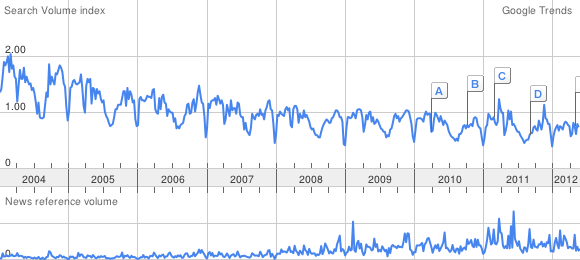
\includegraphics[width=1\linewidth]{google-trends-mobbing.png}}
	\caption{Частота поиска и упоминания в новостях слова mobbing по данным аналитической системы Google Trends.}
	\label{fig:google-trends-mobbing}
\end{figure}

Рассматривая потенциальный вред от разрабатываемой системы, отметим, что все её компоненты являются исключительно программными средствами, а потому физический вред нанести в той же мере, в которой те аппаратные средства, на которых система выполняется. Однако ни в коем случае нельзя оставлять за пределами рассмотрения потенциальный психологический вред. Так, известно наличие в сети Интернет сайтов, таких как 4chan, длительное пребывание на которых, по мнению многих аналитиков\cite{4chan}, может приводить к деформации личности.

К счастью, можно сразу сказать, что система позиционирования транспорта не предполагает взаимодействие между её пользователями, а сама по себе, хоть и использует алгоритмы машинного обучения, не является в достаточной мере интеллектуальной, чтобы наносить психический вред самостоятельно.

Таким образом, имеет смысл рассматривать вред, который может нанести система через ЭВМ. Здесь также можно отметить значительное устаревание имеющихся нормативные документов. Так, основной нормативный документ, описывающий санитарные требования к рабочему месту оператора ЭВМ --- САНПИН 2.2.2/2.4.1340-03\cite{sanpin} уделяет большое внимание вопросу рентгеновского излучения ЭЛТ-мониторов, несмотря на то, что те из них, которые могли сохранить работоспособность до 2012 года, гарантированно относятся к поколению, в котором вся необходимая защита встроена в корпус трубки. С другой стороны, такому явлению, как чтению с экрана, уделено недопустимо мало внимания. Такая характеристика как контрастность вообще не рассматривается, считаются только знаки, как будто они все равноценны. При том, что многие люди действительно не осведомлены о том, что контрастность текста измерять нужно, и делать это в чёрно-белом варианте, в связи с чем недопустим, например, светло-зелёный текст на розовом фоне, хотя эти цвета очень легко различить.

Не уделяется там и внимание такому фактору, давно изучаемому специалистами по интерфейсам, но не специалистами по охране труда, как шрифты. А ведь замечено, что неправильно подобранный шрифт может существенно уменьшить время, которое человек может провести за чтением текста, не устав.

Ещё одним фактором является мерцание и быстрая смена картинки. На это тоже нет никаких нормативов, в связи с чем, зная, что серверная часть разрабатываемой системы будет выводить на экран много текста с большой скоростью, авторам работы остаётся лишь порекомендовать пользователям, во избежание раздражения и покраснения глаз, не злоупотреблять использованием консольного интерфейса сервера, отдавая предпочтение графическому клиенту. Нормировать этот параметр не представляется возможным за отсутствием необходимых норм.

Таким образом, несомненно, можно выделить много потенциально негативных факторов в работе с любым программным продуктом, но те требования, которые были предъявлены 10 лет назад и продолжают предъявляться до сих пор, не соответствуют реальным потребностям повышения юзабилити, не могут быть выполнены и не выполняются в современных условиях, при том, что новые опасные факторы не нормируются или нормируются с большим опозданием.
